\graphicspath{{./ch_carbon_dephasing_purified/figures/}}


\chapter{Storing a quantum state during optical excitation of a quantum network node}
\label{ch:CDP}

\begin{center} 
    \vspace{-1cm} {M.S.~Blok, K. ~van Bemmelen, N.~Kalb, A.~Reiserer, T.H.~Taminiau and R.~Hanson} 
\end{center}

\vspace{0.5cm} 

The ability to locally store a quantum state in a quantum network node while establishing entanglement with a distant node is a crucial prerequisite for implementing entanglement distillation, purification and quantum repeater protocols\cite{Bennett_Phys.Rev.Lett._1996,Campbell_Phys.Rev.Lett._2008,Briegel_Phys.Rev.Lett._1998,Childress_Phys.Rev.Lett._2006}. For quantum network nodes based on NV centers in diamond, nearby $^{13}$C-spins are a prime candidate for such a quantum memory. The challenge is that these nuclear spins have a constant coupling to the optically active electron spin, resulting in possible dephasing of the stored state when the electron is reset multiple times as required for generating remote entanglement. In chapter \ref{ch:CDL} we discussed an analytical model to describe this process and found that nodes with low electron-nuclear coupling strength and fast electron reset are expected to provide the best performance. Here we present preliminary experimental results to test our model in an isotopically purified sample where $^{13}$C-spins with coupling strengths of < 1 kHz can be located and controlled. We find that multiple resets of the electron spin indeed induce dephasing of the nuclear-spin quantum memory and that this process can be suppressed by reducing the electron reset time. While the data qualitatively agrees with our model, the observed dephasing rate is faster than predicted indicating that we are limited by an additional decoherence process. Nonetheless our results show that a $^{13}$C-spin allows for the storage of a quantum state during 200 repetitions with very little loss of fidelity ($99 \%$ fidelity with initial state).
\clearpage

Here we discuss preliminary data to investigate the ability of a weakly coupled $^{13}$C-spin to store a quantum state while optically addressing the electron spin to generate remote entanglement (as presented in chapter \ref{ch:LDE}). Since this protocol \cite{Barrett_Phys.Rev.A_2005,Bernien_Nature_2013} is inherently probabilistic it must be repeated many times until success, requiring the electron spin to be reset before each repetition. Because the exact time of our reset method is uncertain (the optical pumping is a stochastic process) and electron-nuclear interaction is constant, this can induce dephasing of the nuclear spin memory. From the simulations presented in chapter \ref{ch:CDL} we conclude that this dephasing process can be suppressed by using relatively distant $^{13}$C-spins with low hyperfine coupling and implementing a fast reset that minimizes the time-uncertainty. To locate distant $^{13}$C-spins we use an isotopically purified diamond (0.01 $\%$ $^{13}$C) and show that we can control nuclear spins with a hyperfine coupling constant in the order of $\sim$ 200 Hz. We characterize the reset timescale by varying the time and the power of the repumping laser pulse. Finally we measure the dephasing of the nuclear spin as a function of number of times that the electron spin is reinitialized.

\section{Controlling a weakly coupled $^{13}$C-spin in isotopically purified diamond.}

We detect weakly coupled $^{13}$C-spins in the vicinity of an NV center via the electron spin using dynamical decoupling spectroscopy\cite{Taminiau_Phys.Rev.Lett._2012,Zhao_NatNano_2012,Kolkowitz_Phys.Rev.Lett._2012}. In Fig. \ref{fig:cdp-fig1}a we vary the time between $N = 128$ equally spaced $\pi$-pulses on the electron initially prepared in an equal superposition and plot the probability of recovering $m_s = 0$ after a final $\pi$/2-pulse. The observed periodical collapses\cite{Childress_Science_2006} are well explained by the interaction of the electron spin with a $^{13}$C-spin bath in a magnetic field of 22.7 $G$. We align the magnetic field along the quantization axis of the NV-center by minimizing the average of the $m_s = 0 \rightarrow -1$ and $m_s = 0 \rightarrow +1$ transitions. From these measurements we find a magnetic field $B_z = (22.5 \pm 0.1) $ G and $B_x = (2.4 \pm 2) $ G.

In a higher resolution measurement around the second collapse (Fig. \ref{fig:cdp-fig1}b) we observe two additional resonances associated with single $^{13}$C-spins. The location and shape of these resonances are determined by the hyperfine parameters of the carbon spin\cite{Taminiau_Phys.Rev.Lett._2012}. By comparing the data with simulations of the electron-nuclear interaction we estimate hyperfine constants of $A_{\parallel,C} = 220$ Hz and $A_{\perp,C} = 200$ Hz ($A_{\parallel,C} = -1.02$ kHz and $A_{\perp,C} = 190$ Hz) as plotted in red (green). In comparison, previous experiments have demonstrated control of strongly coupled $^{13}$C-spins with interaction strengths between $\sim$ 100 - 1 MHz \cite{Jelezko_Phys.Rev.Lett._2004,Dutt_Science_2007,Pfaff_NatPhys_2013,Neumann_Science_2008} and weakly coupled nuclear spins in the order of 50-30 kHz \cite{Taminiau_NatNano_2014} in natural abundance samples. In isotopically purified samples, manipulation of a strongly coupled 2.6 kHz $^{13}$C-spin was demonstrated\cite{Maurer_Science_2012}.

 \begin{figure*}
	\centering
	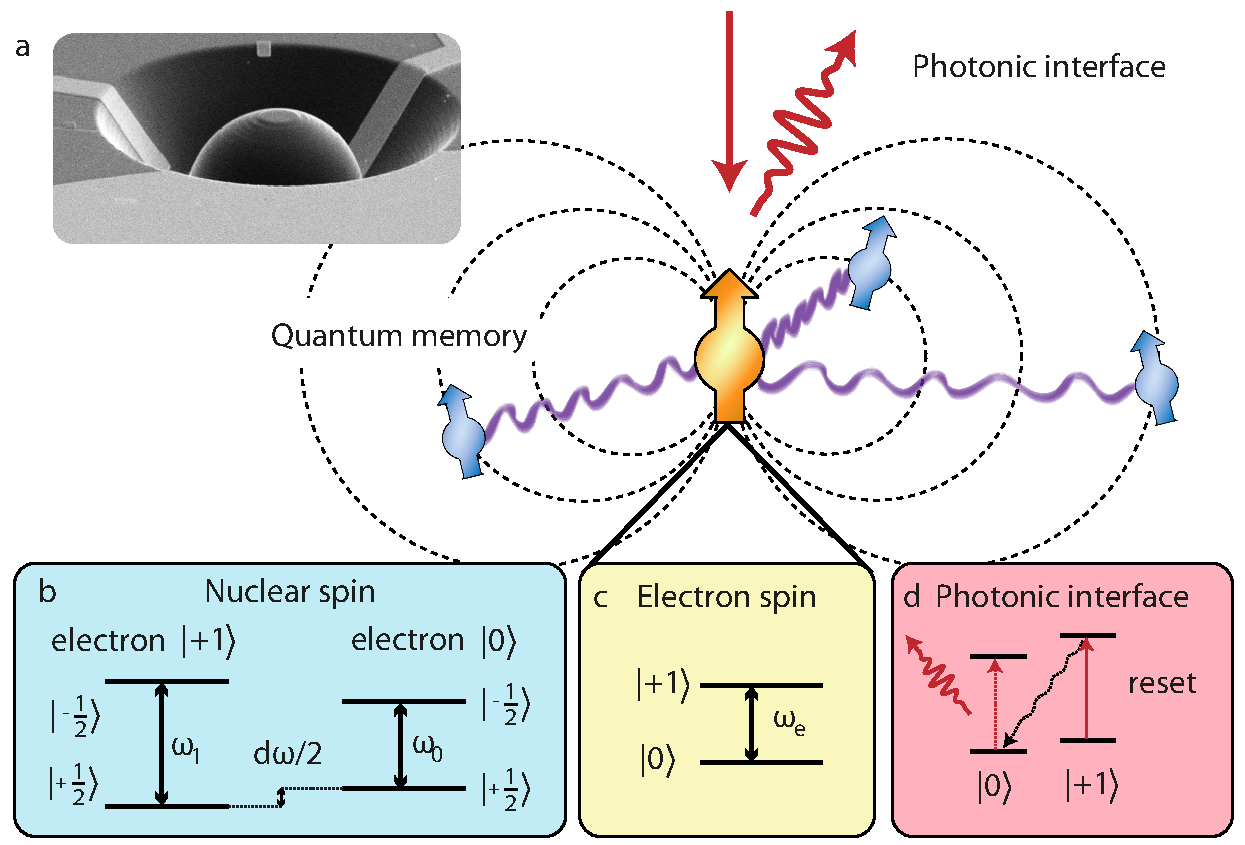
\includegraphics[width=130mm]{Fig1}
	\caption{\label{fig:cdp-fig1} \textbf{} (a) Dynamical Decoupling spectroscopy of the $^{13}$C-spin bath. Grey lines are the expected collapses of the signal due to interaction with the $^{13}$C-spin bath. They occur at $\tau_k = \frac{\pi(2k-1)}{2\omega_L}$, with $\tau_k=1,2,3...$ the order of the resonance and $\omega_L$ the larmor frequency of the $^{13}$C spins.(b) Two $^{13}$C-Spins can be identified, red (green) line is a simulation of the resulting signal for the interaction with a single spin with hyperfine constants of $A_{\parallel,C} = 220$ Hz and $A_{\perp,C} = 200$ Hz ($A_{\parallel,C} = -1.02$ kHz and $A_{\perp,C} = 190$ Hz), plotted in red (green). (c) Free induction decay of a single carbon spin with and without repetitive reset }
\end{figure*}

 \begin{figure*}
	\centering
	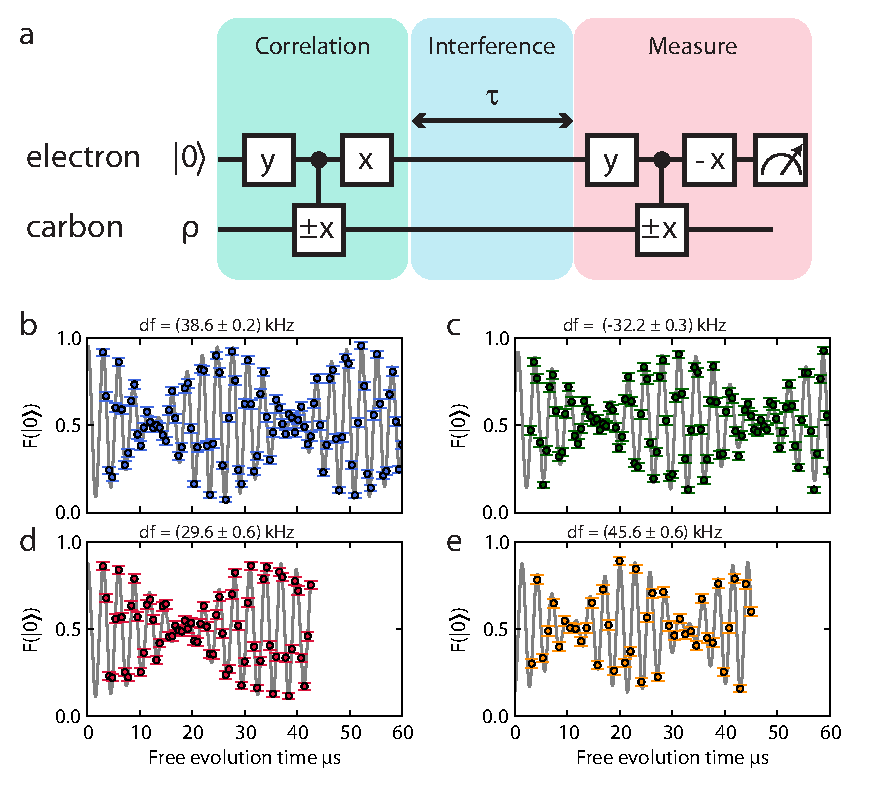
\includegraphics[width=130mm]{Fig2}
	\caption{\label{fig:cdp-fig2} \textbf{Reset of the electron spin} (a) Measurement of the timescale of the reset process. Plotted is the probability of preparing $m_s = 0$ after preparing $m_s = \pm 1$ as a function of repump time and power (b) Fitted time constant of the reset process as a function of reset power.}
\end{figure*}

 \begin{figure*}
	\centering
	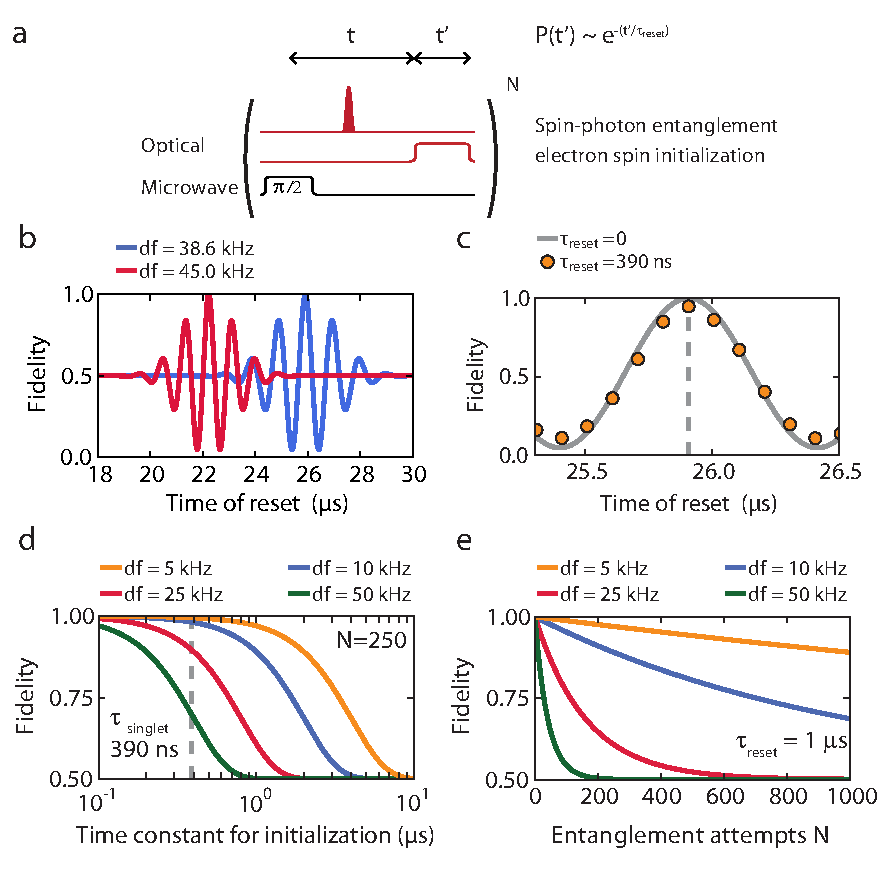
\includegraphics[width=130mm]{Fig3}
	\caption{\label{fig:cdp-fig3} \textbf{} (a) Result of tomography (measuring X,Y and Z) for varying number of resets. (b) }
\end{figure*}

\clearpage
\bibliographystyle{../thesis}
\bibliography{cdp}


